\chapter{Requirements}
\section{Domain analysis}
The domain analysis is carried out by identifying important elements given in the description of the project. The purpose of the analysis is to gain a shared knowledge of the project before starting the development.

\subsection{Domain glossary}
\begin{center}
\begin{table}[!ht]
    \centering
    \begin{tabular}{ | l | p{10cm} | }
    \hline
    \textbf{Item}           &   \textbf{Description} \\ \hline
    Antenna                 &   Antennas is located at the express lane for detecting toll tags on the users vehicle. \\ \hline
    Touchscreen             &   The touchscreen is operated by the cashier at the toll lane. \\ \hline
    Costumer                &   The customer interacts with the system by paying at the toll booths or monthly with the express system. \\ \hline
    Cashier                 &   The cashier operates a single toll booth. \\ \hline
    Enterprise manager      &   The enterprise manager can interact with the system in varies ways, example print reports and change prices for tickets. \\ \hline
    Single ticket reader    &   Only normal check-out lanes has a single ticket reader. \\ \hline
    Barrier                 &   Blocks the road for drivers until they have registered a payment. \\ \hline
    Printer                 &   The printer is only located a normal check-it lanes. \\ \hline
    Credit card reader      &   The credit card reader is only located a normal check-in lanes. \\ \hline
    Toll lane computer      &   The toll lane computer plays many different roles in the system, there exists three types (check-in, check-out and express). \\ \hline
    Toll lane               &   There exists three types of lanes, normal check-in, normal check-out and express lanes. \\ \hline
    Express lane            &   If the user has a toll tag he can use this lane for automatic check-in and check-out. \\ \hline
    Enterprise server       &   The enterprise server consists of several station servers, a client and a web server. \\ \hline
    Web server              &   The web server is used to connect the enterprise system to the Internet. \\ \hline
    Station server          &   A station server consists of several lanes and a client. \\ \hline
    Bank                    &   The software on normal check-in toll lanes is communicating with the bank. \\ \hline
    Toll tag                &   A device the user can purchase for automatic check-in and check-out. \\ \hline
    \end{tabular}
    \caption{Domain glossary}
    \label{tab:bfs_dfs}
\end{table}    
\end{center}

\newpage
\subsection{Domain diagram}
The domain diagram shows the relation between important parts in the system. This is used for finding key points for development, when designing a system.

\begin{figure}[!ht]
  \begin{center}
    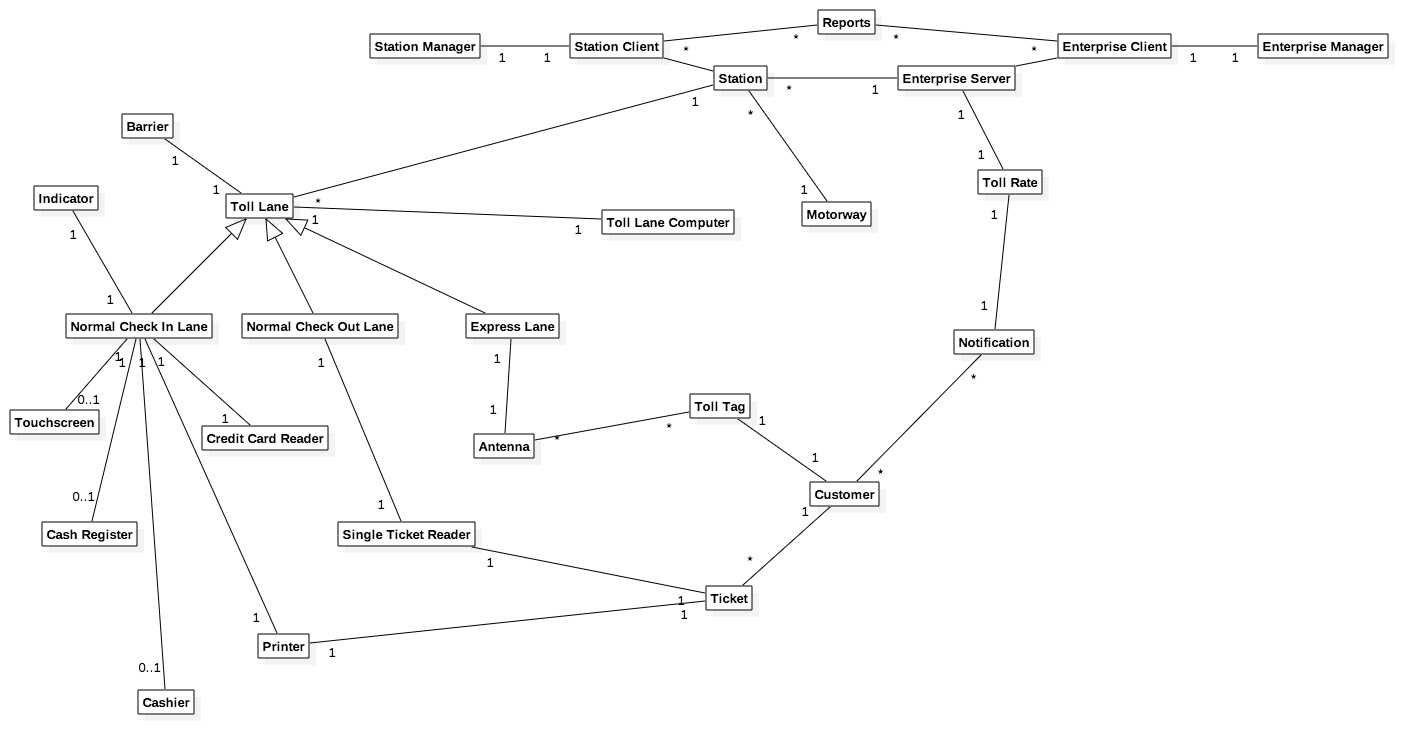
\includegraphics[width=1\textwidth]{figures/domain_model.jpg} 
  \end{center}
  \caption{Domain model diagram for the toll system}
\end{figure}